\documentclass[]{informeutn}
\usepackage{siunitx}
\usepgfplotslibrary{groupplots}

% Paquetes adicionales
\usepackage{csquotes}
\usepackage[backend=bibtex, style=alphabetic, sorting=ynt]{biblatex}
\addbibresource{fuentes.bib}
\usepackage{subcaption}
\usepackage{listings}
\usepackage{pdflscape}
\usepackage{pdfpages}

% We will externalize the figures
\usetikzlibrary{external, calc}
%\tikzexternalize
\tikzset{external/optimize command away=\includepdf}
\pgfplotsset{compat=1.18}

\lstdefinestyle{ltspice}{
  backgroundcolor=\color{gray!10},
  basicstyle=\ttfamily\small,
  keywordstyle=\color{blue},
  frame=single,
  breaklines=true,
  captionpos=b
}

% Datos de la carátula
\materia{Teoria de los Circuitos 2}
\titulo{Trabajo Práctico 1}
%\subtitulo{Analisis, Simulacion e Implementacion de Sistemas Lineales
%e Invariantes en el Tiempo (SLIT)}
\comision{4R2}
\autores{
    Gil, Ignacio - 401891 \\
    Rao, Valentino - 402308
}
%\fecha{19/06/2026}

\begin{document}

\maketitle
\setcounter{page}{1}
\thispagestyle{plain}

\chapter{Introducción}
\label{chap:introduccion}
En el presente informe se desarrolla el Trabajo Práctico Nº 1, cuyo objetivo principal es estudiar y aplicar métodos
de resolución de sistemas lineales e invariantes en el tiempo (SLIT). Para ello, se analizan tres circuitos eléctricos
que representan este tipo de sistemas, abordando su comportamiento tanto desde el punto de vista teórico como práctico.

A lo largo del trabajo se aplican los métodos vistos en clase para resolver los sistemas propuestos, obteniendo sus
respuestas en frecuencia y analizando las características principales de cada circuito. Además, se realizan
simulaciones con el fin de verificar los resultados teóricos y comparar el comportamiento esperado con el obtenido
mediante herramientas computacionales.

Finalmente, se implementan los circuitos de manera experimental y se miden sus respuestas en frecuencia, lo que permite
contrastar los resultados prácticos con los valores calculados y simulados. De esta forma, el trabajo busca integrar
el análisis matemático, la simulación y la implementación física de sistemas SLIT, fortaleciendo la comprensión de su
funcionamiento y sus aplicaciones en circuitos eléctricos.

\chapter{Circuito 1}
\label{chap:circuito_1}

Se muestra en la Figura \ref{plot:circuito_1} el circuito sobre el que se trabajará, que constituye un filtro pasa bajo
de segundo orden. Los valores de los componentes son:

\begin{itemize}
  \item $R_1: \SI{100}{\kilo\ohm}$
  \item $R_2: \SI{182}{\kilo\ohm}$
  \item $C_1: \SI{91}{\pico\farad}$
  \item $C_2: \SI{33}{\pico\farad}$
\end{itemize}

\begin{figure}[!ht]
  \centering
  \begin{tikzpicture}[transform shape]
	% Paths, nodes and wires:
	\draw (-3, -1) to[sinusoidal voltage source, l={$V_{in}$}] (-3, 1);
	\draw (-2.5, 1.75) to[american resistor, l={$R_1$}] (-0.5, 1.75);
	\draw (0, 1) to[capacitor, l_={$C_1$}] (0, -1);
	\draw (0.5, 1.75) to[american resistor, l={$R_2$}] (2.5, 1.75);
	\draw (3, 1) to[capacitor, l_={$C_2$}, v^=$V_{out}$, voltage/distance from node=0, voltage/shift=1.1, voltage=american] (3, -1);
	\draw (-3, 1) -| (-3, 1.75) -- (-2.5, 1.75);
	\draw (-0.5, 1.75) -- (0.5, 1.75);
	\draw (2.5, 1.75) -| (3, 1);
	\draw (3, -1) |- (-3, -1.75) -| (-3, -1);
	\draw (0, -1) -| (0, -1.75);
	\draw (0, 1.75) -| (0, 1);
	\node[circ] at (0, 1.75){};
	\node[circ] at (0, -1.75){};
\end{tikzpicture}

  \caption{Esquematico del circuito 1.}
  \label{plot:circuito_1}
\end{figure}

\section{Analisis}
\label{sec:analisis_circ_1}

Para el analisis se transforma el circuito a su equivalente en laplace como se ve en la Figura
\ref{plot:circuito_1_laplace} y se aplica el metodo sistematico nodal, el cual nos da las matrices de la ecuacion
\ref{eq:circuito_1_matrices}.


\begin{figure}[!ht]
  \centering
  \begin{tikzpicture}[transform shape]
	% Paths, nodes and wires:
	\draw (-3, -1) to[sinusoidal voltage source, l={$V_{in}$}] (-3, 1);
	\draw (-3, 1) -| (-3, 1.75) -- (-2.5, 1.75);
	\draw (-0.5, 1.75) -- (0.5, 1.75);
	\draw (2.5, 1.75) -| (3, 1);
	\draw (3, -1) |- (-3, -1.75) -| (-3, -1);
	\draw (0, -1) -| (0, -1.75);
	\draw (0, 1.75) -| (0, 1);
	\node[circ](N1) at (0, 1.75){} node[anchor=south] at (N1.text){$V_1$};
	\node[circ] at (0, -1.75){};
	\draw (-2.5, 1.75) to[generic, l={$\small \num{100d3}$}] (-0.5, 1.75);
	\draw (0.5, 1.75) to[generic, l={$\small \num{182d3}$}] (2.5, 1.75);
	\draw (3, 1) to[generic, l={$\frac{1}{\num{33d-12} \cdot s}$}] (3, -1);
	\draw (0, 1) to[generic, l={$\frac{1}{\num{91d-12} \cdot s}$}] (0, -1);
	\node[circ, xscale=0.1, yscale=0.1](N2) at (3, 1.75){} node[anchor=south] at (N2.text){$V_{out}$};
	\node[ground] at (0, -1.75){};
\end{tikzpicture}

  \caption{Equivalente en laplace del circuito 1.}
  \label{plot:circuito_1_laplace}
\end{figure}


\begin{equation}
  Y =
\begin{bmatrix}
  Y_{R_1} + Y_{R_2} + Y_{C_1} & -Y_{R_2} \\
  -Y_{R_2} & Y_{R_2} + Y_{C_2}
\end{bmatrix}
\qquad
I =
\begin{bmatrix}
  \frac{V_{in}(s)}{R_1} \\
0
\end{bmatrix}
  \label{eq:circuito_1_matrices}
\end{equation}

Donde:
\begin{itemize}
  \item $Y_{R_1} = \num{10d-6}$
  \item $Y_{R_2} = \num{5.49d-6}$
  \item $Y_{C_1} = \num{91d-12} \cdot s$
  \item $Y_{C_2} = \num{33d-12} \cdot s$
\end{itemize}

Al resolver la ecuación para obtener las tensiones nodales, se tiene que

\begin{equation}
V = Y^{-1} \cdot I
\end{equation}

En particular, la tensión en el nodo de salida \(V_{out}\) corresponde a la primera fila del vector \(V\), resultando:

$$
  V_{out}(s) = \frac{V_{in}(s) \cdot Y_{R_1} \cdot Y_{R_2}}{Y_{C_1} \cdot Y_{C_2} + Y_{C_1} \cdot Y_{R_1} + Y_{C_1} \cdot Y_{R_2} + Y_{R_1} \cdot Y_{R_2}}
$$

Dividiendo por $V_{in}(s)$, reemplazando los valores de las admitancias por los especificados anteriormente y
resolviendo algebraicamente, se llega finalmente la funcion de transferencia vista en la ecuacion \ref{eq:fdt-circuito-1}

\begin{align}
  H(s) &= \frac{\num{1.83d10}}{s^2 + 533134 \cdot s + \num{1.83d10}}\\
  H(s) &= \frac{\num{1.83d10}}{(s + 496214.48)\cdot(s + 36919.52)}
  \label{eq:fdt-circuito-1}
\end{align}


\section{Circuito 2}
\label{chap:circuito_2}

Se muestra en la Figura \ref{plot:circuito_2} el circuito sobre el que se trabajará, que constituye un filtro elimina banda o notch de segundo orden. Los valores de los componentes son:

\begin{itemize}
  \item $R_1: \SI{100}{\kilo\ohm}$
  \item $C_1: \SI{3.18}{\micro\farad}$
  \item $L_1: \SI{31.83}{\milli\henry}$
\end{itemize}

\begin{figure}[H]
  \centering
  \begin{tikzpicture}[transform shape]
	% Paths, nodes and wires:
	\draw (-2, 1) to[sinusoidal voltage source, l={$V_{in}$}] (-2, -1);
	\draw (-0.75, 2) to[american resistor, l={$R_1$}] (1, 2);
	\draw (2, -0) to[american inductor, l={$L_1$}] (2, -2);
	\draw (2, 2) to[capacitor, l={$C_1$}] (2, -0);
	\draw (2, 2) -- (1, 2);
	\draw (-0.75, 2) -| (-2, 1);
	\draw (-2, -1) -| (-2, -2) -- (2, -2);
	\node[ground] at (0, -2){};
	\node[circ, xscale=0.1, yscale=0.1](N1) at (2, 2){} node[anchor=west] at (N1.text){$+  \ \ V_{out}$};
\end{tikzpicture}

  \caption{Esquematico del circuito 2.}
  \label{plot:circuito_2}
\end{figure}

\subsection{Analisis y Simulacion}
\label{sec:analisis_circ_2}

Para el analisis se transforma el circuito a su equivalente en laplace como se ve en la Figura \ref{plot:circuito_2_laplace}.

\begin{figure}[H]
  \centering
  \begin{tikzpicture}[transform shape]
	% Paths, nodes and wires:
	\draw (-2, 1) to[sinusoidal voltage source, l={$V_{in}$}] (-2, -1);
	\draw (2, 2) -- (1, 2);
	\draw (-0.75, 2) -| (-2, 1);
	\draw (-2, -1) -| (-2, -2) -- (2, -2);
	\node[ground] at (0, -2){};
	\draw (-0.75, 2) to[generic, l={$\small 100\ k$}] (1, 2);
	\draw (2, 2) to[generic, l={$\frac{1}{3.18\ \mu\ *\ s}$}] (2, -0);
	\draw (2, -0) to[generic, l={$\small 31.83\ m\ *\ s$}] (2, -2);
	\node[circ, xscale=0.1, yscale=0.1](N1) at (2, 2){} node[anchor=south] at (N1.text){$V_{out}$};
	\node[circ, xscale=0.1, yscale=0.1](N2) at (2, -0){} node[anchor=west] at (N2.text){$V_1$};
\end{tikzpicture}
  \caption{Equivalente en laplace del circuito 2.}
  \label{plot:circuito_2_laplace}
\end{figure}

Considerando la salida en circuito abierto, se puede aplicar la formula del divisor de tension sobre la rama formada por la serie del capacitor $C_1$ y el inductor $L_1$:

\begin{equation}
  V_{out}(s) = V_{in}(s) \cdot \frac{Z_{C_1}(s) + Z_{L_1}(s)}{R_1 + Z_{C_1}(s) + Z_{L_1}(s)}
\end{equation}

donde las impedancias de los componentes son $Z_{C_1}(s) = \frac{1}{s C_1}$ y $Z_{L_1}(s) = s L_1$. Sustituyendo y operando algebraicamente, obtenemos la Funcion de Transferencia (FDT):

\begin{equation}
  H(s) = \frac{s^2 L_1 C_1 + 1}{s^2 L_1 C_1 + s R_1 C_1 + 1}
\end{equation}

Dividiendo el numerador y denominador por el producto $L_1 C_1$, se llega a la forma normalizada estandar de un filtro notch:

\begin{equation}
  H(s) = \frac{s^2 + \frac{1}{L_1 C_1}}{s^2 + s \frac{R_1}{L_1} + \frac{1}{L_1 C_1}}
  \label{eq:fdt-circuito-2-simb}
\end{equation}

Reemplazando por los valores especificados de los componentes:
\begin{itemize}
  \item $L_1 C_1 = \num{31.83d-3} \times \num{3.18d-6} \approx \num{1.0122d-7} \text{ s}^2$
  \item $R_1 C_1 = \num{100d3} \times \num{3.18d-6} = \num{0.318} \text{ s}$
  \item $\omega_0^2 = \frac{1}{L_1 C_1} \approx \num{9.88d6} \text{ rad}^2/\text{s}^2$
  \item $\frac{R_1}{L_1} \approx \num{3.14d6} \text{ rad/s}$
\end{itemize}

De esta forma, se llega finalmente a la ecuacion de la FDT vista en \ref{eq:fdt-circuito-2}:

\begin{equation}
  H(s) = \frac{s^2 + \num{9.88d6}}{s^2 + \num{3.14d6} \cdot s + \num{9.88d6}}
  \label{eq:fdt-circuito-2}
\end{equation}

Los polos del sistema son las raices de la ecuacion caracteristica del denominador:

\begin{equation}
  s^2 + \num{3.14d6} \cdot s + \num{9.88d6} = 0
\end{equation}

Debido a que el termino lineal de amortiguamiento ($\num{3.14d6}$) es extremadamente superior al termino cuadratico medio, el discriminante es marcadamente positivo, lo que nos da dos polos reales, negativos y bien diferenciados (sistema fuertemente sobreamortiguado):

\begin{equation}
  p_1 \approx -\frac{1}{R_1 C_1} = -\num{3.14} \text{ rad/s}
\end{equation}
\begin{equation}
  p_2 \approx -\frac{R_1}{L_1} = -\num{3.14d6} \text{ rad/s}
\end{equation}

Se muestran estos polos graficados en el plano complejo en la Figura \ref{img:polos-plano-circuito-2}. Ambos polos se ubican sobre el eje real izquierdo, lo que garantiza la estabilidad del circuito.

\begin{figure}[H]
  \centering
  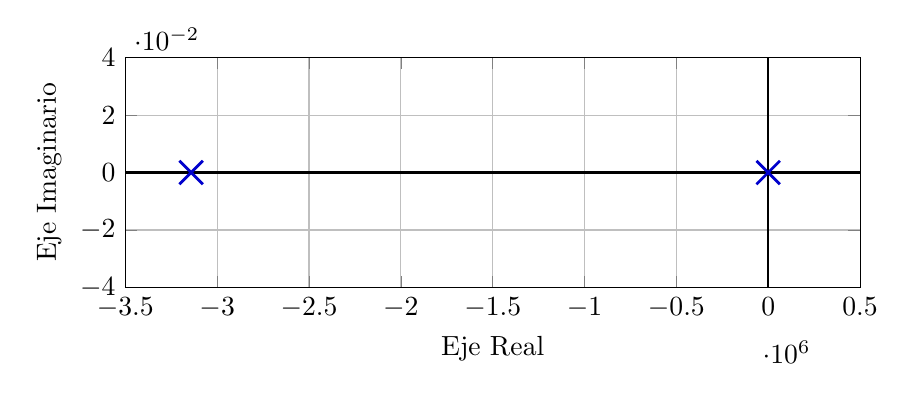
\begin{tikzpicture}
  \begin{axis}[
    width=0.9\columnwidth,
    height=4.5cm,
    xlabel={Eje Real},
    ylabel={Eje Imaginario},
    grid=both,
    xmin=-3500000, xmax=500000,
    ymin=-0.04, ymax=0.04,
  ]
  % Thick x-axis (y=0)
\addplot[
    black,
    line width=0.8pt,
    forget plot
] coordinates {
    (-3500000,0)
    (500000,0)
};

% Thick y-axis (x=0)
\addplot[
    black,
    line width=0.7pt,
    forget plot
] coordinates {
    (0,-0.04)
    (0,0.04)
};

    \addplot[
      scatter,
      only marks,
      mark=x,
      mark size=6pt,
      line width=1pt,
    ]coordinates{
      (-3141690,0)
      (-3.14,0)
    };
  \end{axis}
\end{tikzpicture}

  \caption{Polos en el plano complejo de la FDT del circuito 2.}
  \label{img:polos-plano-circuito-2}
\end{figure}

Se procede ahora a analizar la FDT en el dominio de la frecuencia reemplazando $s = j\omega$, resultando:

\begin{equation}
  H(j\omega) = \frac{1 - \omega^2 L_1 C_1}{1 - \omega^2 L_1 C_1 + j\omega R_1 C_1}
\end{equation}

Para comprobar preliminarmente la validez de la FDT, evaluamos su comportamiento en los extremos de frecuencia:

\begin{align}
  \lim_{\omega \to 0} \frac{1 - \omega^2 L_1 C_1}{1 - \omega^2 L_1 C_1 + j\omega R_1 C_1} &= 1 \\
  \lim_{\omega \to \infty} \frac{1 - \omega^2 L_1 C_1}{1 - \omega^2 L_1 C_1 + j\omega R_1 C_1} &= 1
\end{align}

Esto muestra que las senales de muy baja y muy alta frecuencia pasan sin atenuacion, mientras que a la frecuencia central $\omega_0 = \frac{1}{\sqrt{L_1 C_1}} \approx \num{3143} \text{ rad/s}$ ($f_0 \approx \SI{500}{\hertz}$), la ganancia se anula por completo ($H(j\omega_0) = 0$), confirmando el comportamiento ideal de un filtro notch.

A fin de obtener el diagrama polar de la FDT, separamos la funcion en su parte real e imaginaria multiplicando y dividiendo por el conjugado del denominador:

\begin{align}
  Re(\omega) &= \frac{(1 - \omega^2 L_1 C_1)^2}{(1 - \omega^2 L_1 C_1)^2 + (\omega R_1 C_1)^2} \\
  Img(\omega) &= \frac{-\omega R_1 C_1 (1 - \omega^2 L_1 C_1)}{(1 - \omega^2 L_1 C_1)^2 + (\omega R_1 C_1)^2}
\end{align}

Estas ecuaciones describen geometricamente una circunferencia desplazada en el plano complejo, que cumple con la relacion algebraica:

\begin{equation}
  \left(Re(\omega) - \frac{1}{2}\right)^2 + Img(\omega)^2 = \left(\frac{1}{2}\right)^2
\end{equation}

La Figura \ref{plot:polar_circuito_2} muestra el diagrama polar obtenido de la FDT ideal.

\begin{figure}[H]
  \centering
  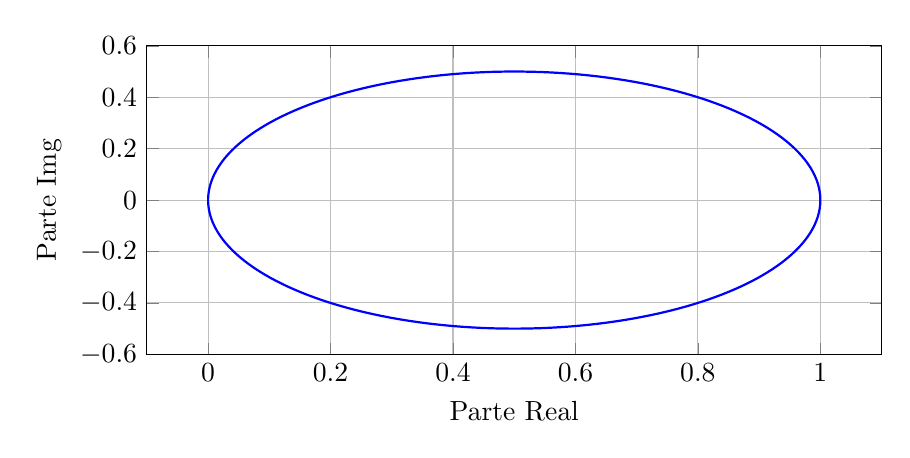
\begin{tikzpicture}
  \begin{axis}[
    width=0.9\columnwidth,
    height=5.5cm,
    xlabel={Parte Real},
    ylabel={Parte Img},
    grid=both,
    xmin=-0.1, xmax=1.1,
    ymin=-0.6, ymax=0.6,
    ytick={-0.6,-0.4,-0.2,0,0.2,0.4,0.6},
    xtick={0,0.2,0.4,0.6,0.8,1.0},
    axis lines=box,
  ]
  \addplot[
      blue,
      thick,
      domain=0:360,
      samples=200,
  ]
  (
      {0.5 + 0.5*cos(x)},
      {0.5*sin(x)}
  );
  \end{axis}
\end{tikzpicture}

  \caption{Diagrama polar de la FDT del circuito 2 (ideal).}
  \label{plot:polar_circuito_2}
\end{figure}

\begin{figure}[H]
  \centering
  \begin{tikzpicture}
\begin{semilogxaxis}[
    xlabel={Frecuencia $\omega$ (rad/s)},
    ylabel={Magnitud (dB)},
    grid=both,
    grid style={line width=.1pt, draw=gray!30},
    major grid style={line width=.2pt, draw=gray!60},
    xmin=1e-1, xmax=1e8,
    ymin=-120, ymax=10,
    width=0.9\columnwidth,
    height=5.5cm,
    legend style={
        at={(0.5, 1.05)}, % x=0.5 (centro horizontal), y=1.05 (por encima del límite superior)
        anchor = south,
        scale = 0.9,
        font=\footnotesize % Reduce el tamaño del texto y los símbolos
    }
]

% Trazado asintótico
\addplot[thick, blue] coordinates {
    (1e-1, 0)
    (3.14, 0)
    (3143, -60)
    (3.14e6, 0)
    (1e8, 0)
};
\addlegendentry{Teórico (Asintótico)}

% Marcador de wp1
\draw[dashed, red, thin] (axis cs:3.14, 0) -- (axis cs:3.14, -60);
\addplot[mark=*, mark size=1.5pt, red, forget plot] coordinates {(3.14, -60)};
\node[anchor=north, font=\scriptsize, text=black] at (axis cs:3.14, -60) {$\omega_{p1} = 3.14$};

% Marcador de w0
\addplot[mark=*, mark size=1.5pt, red, forget plot] coordinates {(3143, -60)};
\node[anchor=south, font=\scriptsize, text=black] at (axis cs:3143, -50) {$\omega_{0} = 3143$};

% Marcador de wp2
\draw[dashed, red, thin] (axis cs:3.14e6, 0) -- (axis cs:3.14e6, -60);
\addplot[mark=*, mark size=1.5pt, red, forget plot] coordinates {(3.14e6, -60)};
\node[anchor=north, font=\scriptsize, text=black] at (axis cs:3.14e6, -60) {$\omega_{p2} = 3.14\text{ M}$};

% Datos de LTSpice
\addplot[thick, dashed, orange] table [
    skip first n=1,
    x expr=\thisrowno{0} * 2 * pi,
    y index=1
] {sim/bode_2.txt};
\addlegendentry{Simulación LTSpice}

\end{semilogxaxis}
\end{tikzpicture}

  \caption{Diagrama de Bode de Magnitud del circuito 2 (Simulado vs Asintótico).}
  \label{plot:bode_mag_circuito_2}
\end{figure}

\begin{figure}[H]
  \centering
  \begin{tikzpicture}
\begin{semilogxaxis}[
    xlabel={Frecuencia $\omega$ (rad/s)},
    ylabel={Fase (grados)},
    grid=both,
    grid style={line width=.1pt, draw=gray!30},
    major grid style={line width=.2pt, draw=gray!60},
    xmin=1e-1, xmax=1e8,
    ymin=-120, ymax=120,
    ytick={-90, 0, 90},
    width=0.9\columnwidth,
    height=5.5cm,
    legend style={
        at={(0.5, 1.05)}, % x=0.5 (centro horizontal), y=1.05 (por encima del límite superior)
        anchor = south,
        scale = 0.9,
        font=\footnotesize % Reduce el tamaño del texto y los símbolos
    }
]

% Trazado asintótico de fase
\addplot[thick, blue] coordinates {
    (1e-1, 0)
    (0.314, 0)
    (31.4, -90)
    (3143, -90)
    (3143, 90)
    (3.14e5, 90)
    (3.14e7, 0)
    (1e8, 0)
};
\addlegendentry{Teórico (Asintótico)}

% Marcas de los polos y ceros
\addplot[mark=|, mark size=3pt, red, forget plot] coordinates {(0.314, 0)};
\node[anchor=south west, font=\small, text=black] at (axis cs:0.314, 0) {$0.1\omega_{p1}$};

\addplot[mark=|, mark size=3pt, red, forget plot] coordinates {(3.14e7, 0)};
\node[anchor=north east, font=\small, text=black] at (axis cs:3.14e7, 0) {$10\omega_{p2}$};

% Datos de LTSpice
\addplot[thick, dashed, orange] table [
    skip first n=1,
    x expr=\thisrowno{0} * 2 * pi,
    y index=2
] {sim/bode_2.txt};
\addlegendentry{Simulación LTSpice}

\end{semilogxaxis}
\end{tikzpicture}

  \caption{Diagrama de Bode de Fase del circuito 2 (Simulado vs Asintótico).}
  \label{plot:bode_phase_circuito_2}
\end{figure}

\subsection{Mediciones de Laboratorio}
\label{sec:mediciones_circ_2}

Para la verificación experimental, se realizó la implementación física del filtro notch utilizando componentes reales cuyos valores medidos fueron:
\begin{itemize}
  \item Resistencia: $R = \SI{100}{\kilo\ohm}$
  \item Inductor: $L = \SI{31.8}{\milli\henry}$
  \item Capacitor: $C = \SI{3.3}{\micro\farad}$
\end{itemize}

El capacitor utilizado en el laboratorio ($C = \SI{3.3}{\micro\farad}$) es muy cercano al valor de diseño teórico de $\SI{3.18}{\micro\farad}$. Con estos componentes reales, la frecuencia angular de resonancia teórica $\omega_0$ y la correspondiente frecuencia de corte $f_0$ son:
\begin{equation}
  \omega_0 = \frac{1}{\sqrt{L \cdot C}} = \frac{1}{\sqrt{\SI{31.8}{\milli\henry} \cdot \SI{3.3}{\micro\farad}}} \approx \SI{3087.96}{\radian\per\second}
\end{equation}
\begin{equation}
  f_0 = \frac{\omega_0}{2\pi} \approx \SI{491.46}{\hertz}
\end{equation}

Los polos del sistema real se ubican teóricamente en:
\begin{align}
  p_1 &\approx -\frac{1}{R \cdot C} = -\SI{3.03}{\radian\per\second} \quad (f_{p1} \approx \SI{0.48}{\hertz}) \\
  p_2 &\approx -\frac{R}{L} = -\SI{3.14}{\mega\radian\per\second} \quad (f_{p2} \approx \SI{500.5}{\kilo\hertz})
\end{align}

Durante el ensayo en el laboratorio, se utilizó un generador de señales para aplicar una tensión senoidal $V_{in}$ a la entrada del filtro. Se midieron las tensiones de entrada y salida con un osciloscopio digital RIGOL. Todas las mediciones de tensión en la Tabla \ref{tab:mediciones_circuito_2} han sido unificadas a valor eficaz ($V_{rms}$) para garantizar la consistencia, realizando la conversión $V_{rms} = V_{pp}/(2\sqrt{2})$ para las frecuencias de \SI{2}{\hertz} y \SI{10}{\hertz} que originalmente se registraron como pico a pico ($V_{pp}$). La atenuación del filtro se expresa directamente como ganancia en decibeles.

\begin{table}[H]
  \centering
  \begin{tabular}{cccc}
    \hline
    \textbf{Frecuencia} & \textbf{Tensión $V_{in}$ ($V_{rms}$)} & \textbf{Tensión $V_{out}$ ($V_{rms}$)} & \textbf{Ganancia [dB]} \\ \hline
    \SI{2}{\hertz}      & \SI{2.40}{\volt}                      & \SI{678.8}{\milli\volt}                 & \SI{-10.98}{\decibel}  \\
    \SI{10}{\hertz}     & \SI{2.62}{\volt}                      & \SI{169.7}{\milli\volt}                 & \SI{-23.76}{\decibel}  \\
    \SI{100}{\hertz}    & \SI{2.5}{\volt}                       & \SI{86}{\milli\volt}                    & \SI{-29.27}{\decibel}  \\
    \SI{1}{\kilo\hertz} & \SI{2.5}{\volt}                       & \SI{90}{\milli\volt}                    & \SI{-28.87}{\decibel}  \\
    \SI{10}{\kilo\hertz}& \SI{2.5}{\volt}                       & \SI{10}{\milli\volt}                    & \SI{-47.96}{\decibel}  \\
    \SI{100}{\kilo\hertz}& \SI{2.5}{\volt}                      & \SI{770}{\milli\volt}                   & \SI{-10.23}{\decibel}  \\
    \SI{200}{\kilo\hertz}& \SI{2.5}{\volt}                      & \SI{1.19}{\volt}                        & \SI{-6.45}{\decibel}   \\ \hline
  \end{tabular}
  \caption{Mediciones experimentales del circuito 2 en el laboratorio (unificadas a valor eficaz).}
  \label{tab:mediciones_circuito_2}
\end{table}

\begin{figure}[H]
  \centering
  \begin{tikzpicture}
\begin{semilogxaxis}[
    title={Comparación de Magnitud del Circuito 2 Real},
    xlabel={Frecuencia $\omega$ (rad/s)},
    ylabel={Magnitud (dB)},
    grid=both,
    grid style={line width=.1pt, draw=gray!30},
    major grid style={line width=.2pt, draw=gray!60},
    xmin=1, xmax=2e6,
    ymin=-80, ymax=5,
    width=0.9\columnwidth,
    height=5.5cm,
    legend style={
        nodes={scale=0.7, transform shape},
        at={(0.05,0.05)},
        anchor=south west
    }
]

% Curva de Simulación de LTSpice con Rser = 50 Ohm y C = 3.3 uF
\addplot[thick, blue] table [
    skip first n=1,
    x expr=\thisrowno{0} * 2 * pi,
    y index=1
] {sim/circuito_2_50omh.txt};
\addlegendentry{Simulación (LTSpice, $R_{ser}=50\,\Omega$)}

% Puntos Medidos en Laboratorio
\addplot[
    only marks,
    mark=*,
    mark size=2.0pt,
    red
] coordinates {
    (12.56637, -10.98)     % 2 Hz
    (62.83185, -23.76)     % 10 Hz
    (628.3185, -29.27)     % 100 Hz
    (6283.185, -28.87)     % 1 kHz
    (62831.85, -47.96)     % 10 kHz
    (628318.53, -10.23)    % 100 kHz
    (1256637.06, -6.45)    % 200 kHz
};
\addlegendentry{Mediciones de Laboratorio}

\end{semilogxaxis}
\end{tikzpicture}

  \caption{Comparación entre la simulación de LTSpice del circuito real (con $C = \SI{3.3}{\micro\farad}$ y $R_{ser} = \SI{50}{\ohm}$ para modelar la pérdida del inductor) y las mediciones obtenidas en el laboratorio.}
  \label{plot:bode_medido_vs_teorico_circuito_2}
\end{figure}

A partir de las mediciones graficadas en la Figura \ref{plot:bode_medido_vs_teorico_circuito_2}, se observa un buen acuerdo general con la respuesta simulada. A frecuencias muy bajas (\SI{2}{\hertz} y \SI{10}{\hertz}) y altas (\SI{100}{\kilo\hertz} y \SI{200}{\kilo\hertz}), los puntos coinciden notablemente con la simulación. En el rango de \SI{100}{\hertz} a \SI{1}{\kilo\hertz}, los valores medidos presentan una meseta en torno a los \SI{-29}{\decibel}, limitados principalmente por el piso de ruido del instrumental, pero registrando el comportamiento atenuador central esperado.

Para registrar con mayor resolución la respuesta en frecuencia completa del filtro en el entorno de la sintonía, se capturó la pantalla del osciloscopio mostrada en la Figura \ref{img:bode_medido_circuito_2}, la cual grafica la respuesta obtenida mediante la Transformada Rápida de Fourier (FFT). El osciloscopio se configuró con una escala de magnitud vertical de \SI{10.0}{\decibel\text{Vrms}/div} y una escala de frecuencia horizontal de \SI{250.0}{\hertz/div}. Con el inicio del barrido en corriente continua, la fosa del notch se ubicó exactamente a dos divisiones del origen de frecuencias, lo cual corresponde a una frecuencia de sintonía de sintonía de $2 \times \SI{250}{\hertz/div} = \SI{500}{\hertz}$, en excelente concordancia con la frecuencia de resonancia teórica calculada de $\SI{491.46}{\hertz}$. Utilizando los cursores del osciloscopio, se midió un nivel de referencia en la banda de paso de $CurA = \SI{-43.6}{\decibel}$ y el punto mínimo del notch en $CurB = \SI{-74.8}{\decibel}$, registrando una profundidad de notch de $\SI{31.2}{\decibel}$. Este comportamiento práctico valida satisfactoriamente el análisis teórico propuesto para este filtro.

\begin{figure}[H]
  \centering
  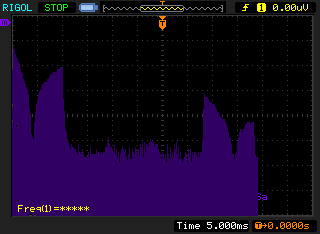
\includegraphics[width=0.8\columnwidth]{images/bd2.png}
  \caption{Respuesta en frecuencia (FFT) del circuito notch real medida en el laboratorio.}
  \label{img:bode_medido_circuito_2}
\end{figure}

\section{Circuito 3}
\label{chap:circuito_3}

Se muestra en la Figura \ref{plot:circuito_3} el circuito sobre el que se trabajará, que constituye un filtro pasa banda
implementado con un amplificador operacional en configuración inversora. Los valores ideales de los componentes dados en el trabajo práctico son:

\begin{itemize}
  \item $R_1: \SI{20}{\kilo\ohm}$
  \item $R_2: \SI{400}{\kilo\ohm}$
  \item $C_1: \SI{1.25}{\micro\farad}$
  \item $C_2: \SI{15.625}{\nano\farad}$
\end{itemize}

\begin{figure}[H]
  \centering
  \begin{tikzpicture}[transform shape, american voltages]
	% Paths, nodes and wires:
	\node[op amp](N1) at (1.56, -0){} node[anchor=center] at (N1.text){$OP1$};
	\draw (0.25, 4) to[american resistor, l_={$R_2$}] (2.75, 4);
	\draw (0.25, 2) to[capacitor, l_={$C_2$}] (2.75, 2);
	\draw (2.75, 0) -- (3.75, 0) -| (3.75, 2) |- (2.75, 3);
	\draw (2.75, 4) -| (2.75, 2);
	\draw (0.25, 4) -- (0.25, 2);
	\draw (-1.5, 3) to[capacitor, l={$C_1$}] (-2.5, 3);
	\draw (-3.25, 2) to[american resistor, l={$R_1$}] (-3.25, 0.5);
	\draw (-3.25, -0.25) to[sinusoidal voltage source, l={$V_{in}$}] (-3.25, -1.75);
	\draw (-3.25, -0.25) -| (-3.25, 0.5);
	\draw (-3.25, 2) -| (-3.25, 3);
	\draw (0.37, 0.49) -| (-1, 3);
	\draw (0.37, -0.49) |- (-3.25, -2) -| (-3.25, -1.75);
	\node[ground] at (0.37, -2){};
	\node[circ] at (2.75, 3){};
	\node[circ] at (0.25, 3){};
	\node[circ] at (-1, 3){};
	\node[circ, xscale=0.1, yscale=0.1](N2) at (3.75, -0){} node[anchor=west] at ([xshift=0.06cm]N2.text){$+ \ \ V_{out}$};
	\node[circ] at (0.37, -2){};
	\draw (-3.25, 3) -- (-2.5, 3);
	\draw (-1.5, 3) -- (0.25, 3);
\end{tikzpicture}

  \caption{Esquemático del circuito 3.}
  \label{plot:circuito_3}
\end{figure}

\subsection{Análisis y Simulación (Ideal)}
\label{sec:analisis_circ_3_ideal}

Para el análisis matemático de este circuito, se obtienen primero las impedancias de la rama de entrada ($Z_i$) y de la rama de realimentación ($Z_f$). 
La impedancia de entrada corresponde a la combinación en serie de $R_1$ y $C_1$:
\begin{equation}
  Z_i(s) = R_1 + \frac{1}{s C_1} = \frac{1 + s R_1 C_1}{s C_1}
\end{equation}

La impedancia de realimentación es el paralelo entre $R_2$ y $C_2$:
\begin{equation}
  Z_f(s) = \left( \frac{1}{R_2} + s C_2 \right)^{-1} = \frac{R_2}{1 + s R_2 C_2}
\end{equation}

Dado que el amplificador operacional se encuentra en configuración inversora, la función de transferencia general se define como:
\begin{equation}
  H(s) = \frac{V_{out}(s)}{V_{in}(s)} = -\frac{Z_f(s)}{Z_i(s)}
\end{equation}

Reemplazando las expresiones de las impedancias:
\begin{equation}
  \label{eq:fdt-circuito-3-generica}
  H(s) = -\frac{\frac{R_2}{1 + s R_2 C_2}}{\frac{1 + s R_1 C_1}{s C_1}} = -\frac{s R_2 C_1}{(1 + s R_1 C_1)(1 + s R_2 C_2)}
\end{equation}

Expandiendo el denominador obtenemos la forma genérica polinómica:
\begin{equation}
  H(s) = -\frac{s R_2 C_1}{s^2 R_1 R_2 C_1 C_2 + s (R_1 C_1 + R_2 C_2) + 1}
\end{equation}

Reemplazando por los valores ideales ($R_1 = \SI{20}{\kilo\ohm}$, $R_2 = \SI{400}{\kilo\ohm}$, $C_1 = \SI{1.25}{\micro\farad}$, $C_2 = \SI{15.625}{\nano\farad}$), obtenemos:
\begin{align}
  H(s) &= -\frac{0.5 s}{(1 + 0.025 s)(1 + 0.00625 s)}\\
  H(s) &= -\frac{0.5 s}{\num{1.5625d-4} s^2 + 0.03125 s + 1}
\end{align}

Dividiendo numerador y denominador por el coeficiente principal del denominador ($\num{1.5625d-4}$), se llega a la Función de Transferencia en su forma canónica:
\begin{align}
  \label{eq:fdt-circuito-3-ideal}
  H(s) &= -\frac{3200 s}{s^2 + 200 s + 6400}\\
  H(s) &= -\frac{3200 s}{(s + 40)(s + 160)}
  \label{eq:fdt-circuito-3-simplify}
\end{align}

Los polos se ubican en $s = -40$ rad/s y $s = -160$ rad/s. Ambos polos son reales y negativos, indicando que el sistema es estable.

\begin{figure}[H]
  \centering
  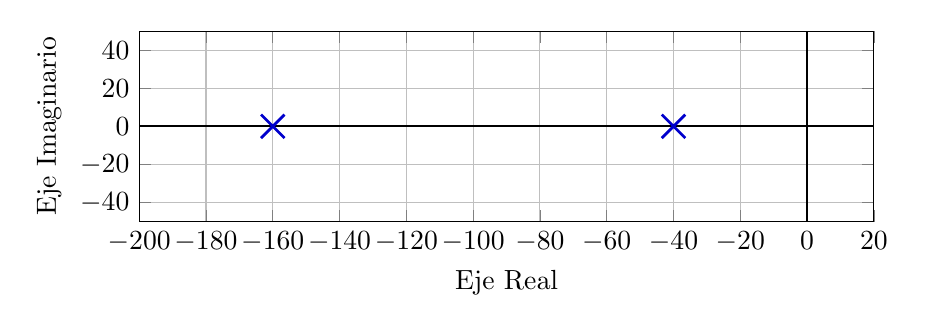
\begin{tikzpicture}
  \begin{axis}[
    width=0.9\columnwidth,
    height=4cm,
    xlabel={Eje Real},
    ylabel={Eje Imaginario},
    grid=both,
    xmin=-200, xmax=20,
    ymin=-50, ymax=50,
  ]
  % Thick x-axis (y=0)
\addplot[
    black,
    line width=0.8pt,
    forget plot
] coordinates {
    (-200,0)
    (20,0)
};

% Thick y-axis (x=0)
\addplot[
    black,
    line width=0.7pt,
    forget plot
] coordinates {
    (0,-50)
    (0,50)
};

    \addplot[
      scatter,
      only marks,
      mark=x,
      mark size=6pt,
      line width=1pt,
      blue,
    ]coordinates{
      (-160,0)
      (-40,0)
    };
  \end{axis}
\end{tikzpicture}

  \caption{Polos en el plano complejo de la FDT.}
  \label{plot:poles_circuito_3}
\end{figure}

Se procede ahora a analizar la FDT en el dominio de la frecuencia reemplazando $s = j\omega$:
\begin{align}
  H(j\omega) &= -\frac{3200 \cdot j\omega}{(j\omega)^2 + 200 \cdot j\omega + 6400} \\
             &= \frac{-3200 \cdot j\omega}{-\omega^2 + 200 \cdot j\omega + 6400}
  \label{eq:fdt-dominio-freq-circuito-3}
\end{align}

Para evaluar los límites de la función de transferencia:
\begin{equation}
  \lim_{\omega \to 0} H(j\omega) = 0
  \qquad \text{y} \qquad
  \lim_{\omega \to \infty} H(j\omega) = 0
\end{equation}
Este comportamiento es el esperado para un filtro pasa banda.

Para el diagrama polar, se separa $H(j\omega)$ en sus componentes real e imaginaria multiplicando y dividiendo por el conjugado del denominador:
\begin{align}
  Re(\omega) &= - \frac{640000 \cdot \omega^2}{\omega^4 + 27200 \cdot \omega^2 + 40960000}\\
  Img(\omega) &= - \frac{3200 \cdot \omega \cdot (6400 - \omega^2)}{\omega^4 + 27200 \cdot \omega^2 + 40960000}
\end{align}

% TODO: El usuario insertará la imagen sacada de LTSpice para el diagrama polar. Se deja el espacio comentado.
\begin{figure}[H]
  \centering
  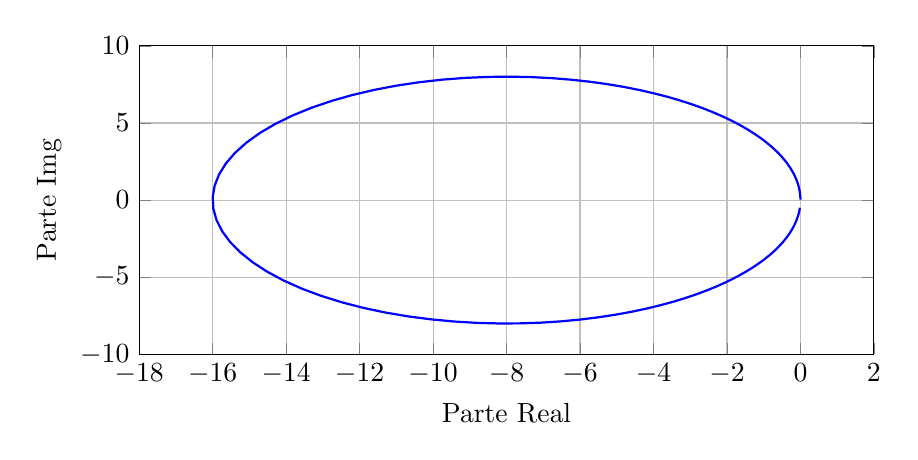
\begin{tikzpicture}
  \begin{axis}[
    width=0.9\columnwidth,
    height=5.5cm,
    xlabel={Parte Real},
    ylabel={Parte Img},
    grid=both,
    xmin=-18, xmax=2,
    ymin=-10, ymax=10,
  ]
  
  \addplot [
    domain=0:5,
    samples=200,
    variable=\t,
    color=blue,
    thick,
  ] (
    { - (640000 * (10^\t)^2) / ((10^\t)^4 + 27200 * (10^\t)^2 + 40960000) },
    { - (3200 * (10^\t) * (6400 - (10^\t)^2)) / ((10^\t)^4 + 27200 * (10^\t)^2 + 40960000) }
  );

  \end{axis}
\end{tikzpicture}

  % \includegraphics[width=0.9\columnwidth]{images/polar_3.png}
  \caption{Diagrama polar de la FDT (Ideal).}
  \label{plot:polar_circuito_3_ideal}
\end{figure}

\begin{figure}[H]
  \centering
  \begin{tikzpicture}
\begin{semilogxaxis}[
    title={Diagrama de Bode de Magnitud},
    xlabel={Frecuencia $\omega$ (rad/s)},
    ylabel={Magnitud (dB)},
    grid=both,
    grid style={line width=.1pt, draw=gray!30},
    major grid style={line width=.2pt, draw=gray!60},
    xmin=1e0, xmax=1e5,
    ymin=-40, ymax=40,
    width=0.9\columnwidth,
    height=8cm,
    legend style={
    nodes={scale=0.7, transform shape}
}
]

\addplot[thick, blue] coordinates {
    (1, -6.02)
    (40, 26.02)
    (160, 26.02)
    (1e5, -29.90)
};
\addlegendentry{Teórico (Asintótico)}

\addplot[mark=*, mark size=1.5pt, red, forget plot] coordinates {(40, 26.02)};
\node[anchor=south east, font=\small, text=black] at (axis cs:40, 26.02) {$\omega_{p1} = 40$};

\addplot[mark=*, mark size=1.5pt, red, forget plot] coordinates {(160, 26.02)};
\node[anchor=south west, font=\small, text=black] at (axis cs:160, 26.02) {$\omega_{p2} = 160$};

% Datos de LTSpice
\addplot[thick, dashed, orange] table [
    skip first n=1,
    x expr=\thisrowno{0} * 2 * pi,
    y index=1
] {sources/circuito3_cleaned.txt};
\addlegendentry{Simulación LTSpice}

\end{semilogxaxis}
\end{tikzpicture}

  \caption{Diagrama de Bode de Magnitud (Real vs Asintótico Ideal).}
  \label{plot:bode_mag_circuito_3}
\end{figure}

\begin{figure}[H]
  \centering
  \begin{tikzpicture}
\begin{semilogxaxis}[
    xlabel={Frecuencia $\omega$ (rad/s)},
    ylabel={Fase (grados)},
    grid=both,
    grid style={line width=.1pt, draw=gray!30},
    major grid style={line width=.2pt, draw=gray!60},
    xmin=1e0, xmax=1e5,
    ymin=-300, ymax=0,
    ytick={0, -90, -180, -270},
    width=0.9\columnwidth,
    height=4.2cm,
    legend style={
    nodes={scale=0.7, transform shape}
}
]

\addplot[thick, blue] coordinates {
    (1, -90)
    (4, -90)
    (16, -117.09)
    (400, -242.90)
    (1600, -270)
    (1e5, -270)
};
\addlegendentry{Teórico (Asintótico)}

\addplot[mark=|, mark size=3pt, red, forget plot] coordinates {(4, -90)};
\node[anchor=south west, font=\small, text=black] at (axis cs:4, -90) {$0.1\omega_{p1}$};

\addplot[mark=|, mark size=3pt, red, forget plot] coordinates {(16, -117.09)};
\node[anchor=south west, font=\small, text=black] at (axis cs:16, -117.09) {$0.1\omega_{p2}$};

% Datos de LTSpice
\addplot[thick, dashed, orange] table [
    skip first n=1,
    x expr=\thisrowno{0} * 2 * pi,
    y index=2
] {sources/circuito3_cleaned.txt};
\addlegendentry{Simulación LTSpice}

\end{semilogxaxis}
\end{tikzpicture}

  \caption{Diagrama de Bode de Fase (Real vs Asintótico Ideal).}
  \label{plot:bode_phase_circuito_3}
\end{figure}


\subsection{Mediciones de Laboratorio}
\label{sec:mediciones_circ_3}

Para la verificación experimental, se realizó la implementación física del filtro pasa banda utilizando componentes reales cuyos valores medidos fueron:
\begin{itemize}
  \item Resistencia $R_1$: $\SI{20}{\kilo\ohm}$ (construida mediante dos resistencias de $\SI{10}{\kilo\ohm}$ en serie)
  \item Resistencia $R_2$: $\SI{400}{\kilo\ohm}$ (construida mediante una resistencia de $\SI{390}{\kilo\ohm}$ y una de $\SI{10}{\kilo\ohm}$ en serie)
  \item Capacitor $C_1$: $\SI{1.2}{\micro\farad}$
  \item Capacitor $C_2$: $\SI{15}{\nano\farad}$
\end{itemize}

El circuito activo fue montado en protoboard utilizando el amplificador operacional JFET dual \textbf{TL082}.

Los capacitores utilizados en el laboratorio ($C_1 = \SI{1.2}{\micro\farad}$ y $C_2 = \SI{15}{\nano\farad}$) son muy cercanos a los valores de diseño teóricos de $\SI{1.25}{\micro\farad}$ y $\SI{15.625}{\nano\farad}$, respectivamente. Con estos componentes reales, la frecuencia angular central teórica $\omega_0$ y la correspondiente frecuencia central de sintonía $f_0$ son:
\begin{align}
  \omega_0 &= \frac{1}{\sqrt{R_1 \cdot C_1 \cdot R_2 \cdot C_2}} \\
           &= \frac{1}{\sqrt{\SI{20}{\kilo\ohm} \cdot \SI{1.2}{\micro\farad} \cdot \SI{400}{\kilo\ohm} \cdot \SI{15}{\nano\farad}}} \approx \SI{83.33}{\radian\per\second}
\end{align}
\begin{equation}
  f_0 = \frac{\omega_0}{2\pi} \approx \SI{13.26}{\hertz}
\end{equation}

Los polos del sistema real se ubican teóricamente en:
\begin{align}
  p_1 &= -\frac{1}{R_1 \cdot C_1} = -\SI{41.67}{\radian\per\second} \quad (f_{p1} \approx \SI{6.63}{\hertz}) \\
  p_2 &= -\frac{1}{R_2 \cdot C_2} = -\SI{166.67}{\radian\per\second} \quad (f_{p2} \approx \SI{26.53}{\hertz})
\end{align}

Durante el ensayo en el laboratorio, se utilizó un generador de señales para aplicar una tensión senoidal $V_{in}$ a la entrada del filtro. Se midieron las tensiones de entrada y salida con un osciloscopio digital RIGOL. Las mediciones originales se registraron en valor pico a pico ($V_{pp}$), con $V_{in} = \SI{2.64}{\volt}_{pp}$ constante para todas las frecuencias. Para la Tabla \ref{tab:mediciones_circuito_3}, los valores fueron convertidos a valor eficaz mediante $V_{rms} = V_{pp}/(2\sqrt{2})$. La ganancia del filtro se expresa directamente en decibeles.

\begin{table}[H]
  \centering
  \begin{tabular}{cccc}
    \hline
    \textbf{Frecuencia} & \textbf{Tensión $V_{in}$ ($V_{rms}$)} & \textbf{Tensión $V_{out}$ ($V_{rms}$)} & \textbf{Ganancia [dB]} \\ \hline
    \SI{1}{\hertz}       & \SI{0.93}{\volt}                      & \SI{1.70}{\volt}                       & \SI{5.19}{\decibel}    \\
    \SI{2}{\hertz}       & \SI{0.93}{\volt}                      & \SI{1.87}{\volt}                       & \SI{6.02}{\decibel}    \\
    \SI{5}{\hertz}       & \SI{0.93}{\volt}                      & \SI{1.92}{\volt}                       & \SI{6.28}{\decibel}    \\
    \SI{8}{\hertz}       & \SI{0.93}{\volt}                      & \SI{1.92}{\volt}                       & \SI{6.28}{\decibel}    \\
    \SI{10}{\hertz}      & \SI{0.93}{\volt}                      & \SI{1.87}{\volt}                       & \SI{6.02}{\decibel}    \\
    \SI{15}{\hertz}      & \SI{0.93}{\volt}                      & \SI{1.75}{\volt}                       & \SI{5.48}{\decibel}    \\
    \SI{20}{\hertz}      & \SI{0.93}{\volt}                      & \SI{1.64}{\volt}                       & \SI{4.90}{\decibel}    \\
    \SI{25}{\hertz}      & \SI{0.93}{\volt}                      & \SI{1.50}{\volt}                       & \SI{4.11}{\decibel}    \\
    \SI{30}{\hertz}      & \SI{0.93}{\volt}                      & \SI{1.41}{\volt}                       & \SI{3.61}{\decibel}    \\
    \SI{45}{\hertz}      & \SI{0.93}{\volt}                      & \SI{1.13}{\volt}                       & \SI{1.67}{\decibel}    \\
    \SI{60}{\hertz}      & \SI{0.93}{\volt}                      & \SI{0.93}{\volt}                       & \SI{0.00}{\decibel}    \\
    \SI{70}{\hertz}      & \SI{0.93}{\volt}                      & \SI{0.79}{\volt}                       & \SI{-1.43}{\decibel}   \\
    \SI{90}{\hertz}      & \SI{0.93}{\volt}                      & \SI{0.68}{\volt}                       & \SI{-2.77}{\decibel}   \\
    \SI{120}{\hertz}     & \SI{0.93}{\volt}                      & \SI{0.57}{\volt}                       & \SI{-4.35}{\decibel}   \\
    \SI{200}{\hertz}     & \SI{0.93}{\volt}                      & \SI{0.35}{\volt}                       & \SI{-8.43}{\decibel}   \\
    \SI{500}{\hertz}     & \SI{0.93}{\volt}                      & \SI{0.14}{\volt}                       & \SI{-16.39}{\decibel}  \\
    \SI{1}{\kilo\hertz}  & \SI{0.93}{\volt}                      & \SI{0.11}{\volt}                       & \SI{-18.89}{\decibel}  \\
    \SI{1}{\mega\hertz}  & \SI{0.93}{\volt}                      & \SI{0.08}{\volt}                       & \SI{-20.83}{\decibel}  \\ \hline
  \end{tabular}
  \caption{Mediciones experimentales del circuito 3 en el laboratorio (convertidas a valor eficaz).}
  \label{tab:mediciones_circuito_3}
\end{table}

\begin{figure}[H]
  \centering
  \begin{tikzpicture}
\begin{semilogxaxis}[
    title={Comparación de Magnitud del Circuito 3 Real},
    xlabel={Frecuencia $\omega$ (rad/s)},
    ylabel={Magnitud (dB)},
    grid=both,
    grid style={line width=.1pt, draw=gray!30},
    major grid style={line width=.2pt, draw=gray!60},
    xmin=1e-1, xmax=1e7,
    ymin=-60, ymax=30,
    width=0.9\columnwidth,
    height=5.5cm,
    legend pos=north east,
    legend style={
        nodes={scale=0.7, transform shape}
    }
]

% Curva de Simulación de LTSpice con Componentes Reales
\addplot[thick, blue] table [
    skip first n=1,
    x expr=\thisrowno{0} * 2 * pi,
    y index=3
] {sources/circuito3_cleaned.txt};
\addlegendentry{Simulación (LTSpice, Real)}

% Puntos Medidos en Laboratorio
\addplot[
    only marks,
    mark=*,
    mark size=2.0pt,
    red
] coordinates {
    (6.283, 5.19)          % 1 Hz
    (12.566, 6.02)         % 2 Hz
    (31.416, 6.28)         % 5 Hz
    (50.265, 6.28)         % 8 Hz
    (62.832, 6.02)         % 10 Hz
    (94.248, 5.48)         % 15 Hz
    (125.664, 4.90)        % 20 Hz
    (157.080, 4.11)        % 25 Hz
    (188.496, 3.61)        % 30 Hz
    (282.743, 1.67)        % 45 Hz
    (376.991, 0.00)        % 60 Hz
    (439.823, -1.43)       % 70 Hz
    (565.487, -2.77)       % 90 Hz
    (753.982, -4.35)       % 120 Hz
    (1256.637, -8.43)      % 200 Hz
    (3141.593, -16.39)     % 500 Hz
    (6283.185, -18.89)     % 1 kHz
    (6283185.307, -20.83)  % 1 MHz
};
\addlegendentry{Mediciones de Laboratorio}

\end{semilogxaxis}
\end{tikzpicture}

  \caption{Comparación entre la simulación de LTSpice del circuito real y las mediciones obtenidas en el laboratorio.}
  \label{plot:bode_medido_vs_teorico_circuito_3}
\end{figure}

A partir de las mediciones graficadas en la Figura \ref{plot:bode_medido_vs_teorico_circuito_3}, se observa el comportamiento característico de un filtro pasa banda. La ganancia máxima medida es de \SI{6.28}{\decibel}, alcanzada entre \SI{5}{\hertz} y \SI{8}{\hertz}, lo que ubica la frecuencia central experimental del filtro en dicho rango. A frecuencias superiores, la atenuación crece progresivamente con una pendiente cercana a \SI{-20}{\decibel} por década, registrándose \SI{-18.89}{\decibel} a \SI{1}{\kilo\hertz} y \SI{-20.83}{\decibel} a \SI{1}{\mega\hertz}.

Para registrar con mayor resolución la respuesta en frecuencia completa del filtro, se capturó la pantalla del osciloscopio mostrada en la Figura \ref{img:fft_circuito_3}, la cual grafica la respuesta obtenida mediante la Transformada Rápida de Fourier (FFT).

\begin{figure}[H]
  \centering
  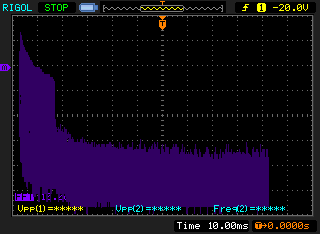
\includegraphics[width=0.9\columnwidth]{images/b3.png}
  \caption{FFT y barrido de frecuencia medido en el laboratorio.}
  \label{img:fft_circuito_3}
\end{figure}


\section{Desarrollo de Herramienta en Octave}
\label{chap:codigo_octave}

Para facilitar la verificación de los diagramas de Bode (tanto asíntotas como curvas reales) y el diagrama polar de manera ágil durante las sesiones de laboratorio, se desarrolló un script en el lenguaje Octave. Dicho script permite al usuario ingresar los coeficientes de los polinomios del numerador y denominador de cualquier función de transferencia $H(s)$ y genera automáticamente las gráficas de respuesta en frecuencia.

El código hace uso del paquete \texttt{control} de Octave para definir la función de transferencia y llama a la librería de terceros \texttt{bodas.m} para el trazado preciso de las asíntotas, además de utilizar las funciones nativas para el diagrama de Nyquist (Polar).

El código fuente del script desarrollado se detalla en el Listado \ref{lst:rao_bodes}.

\lstset{
  literate={á}{{\'a}}1 {é}{{\'e}}1 {í}{{\'i}}1 {ó}{{\'o}}1 {ú}{{\'u}}1
           {Á}{{\'A}}1 {É}{{\'E}}1 {Í}{{\'I}}1 {Ó}{{\'O}}1 {Ú}{{\'U}}1
           {ñ}{{\~n}}1 {Ñ}{{\~N}}1 {¡}{{!`}}1 {¿}{{?`}}1
}
\begin{lstlisting}[float=*, language=Matlab, caption={Script de Análisis de Función de Transferencia en Octave (\texttt{rao\_bodes.m}).}, label={lst:rao_bodes}, frame=tb, breaklines=true, showstringspaces=false, basicstyle=\ttfamily\scriptsize, numbers=left, numberstyle=\tiny, keywordstyle=\color{blue}, commentstyle=\color{green!50!black}, stringstyle=\color{red}, xleftmargin=2em, framexleftmargin=1.5em]
% -------------------------------------------------------------------
% Cátedra: Teoría de Circuitos II - UTN FRC
% Script de Análisis de Función de Transferencia Universal
% Utiliza la librería "bodas" para trazar asíntotas exactas.
% -------------------------------------------------------------------

clear; clc; close all;

% Intentamos cargar el paquete de control, necesario para la función tf()
try
    pkg load control;
catch
    warning('El paquete "control" no está instalado o cargado. Puede fallar si no se usa MATLAB.');
end

fprintf('=======================================================\n');
fprintf('  Análisis de H(s) con Trazado Asintótico (Repo: bodas)\n');
fprintf('=======================================================\n\n');

fprintf('Ingrese los polinomios de la Función de Transferencia H(s).\n');
fprintf('Use el formato de vector de coeficientes descendentes en "s".\n');
fprintf('Ejemplo: para s^2 + 200s + 6400, ingrese [1 200 6400]\n\n');

% 1. Ingreso de datos por parte del usuario
num = input('Ingrese el vector del NUMERADOR: ');
den = input('Ingrese el vector del DENOMINADOR: ');

% 2. Creación del sistema
H = tf(num, den);

fprintf('\n-------------------------------------------------------\n');
fprintf('FUNCIÓN DE TRANSFERENCIA H(s) INGRESADA:\n');
display(H);
fprintf('-------------------------------------------------------\n\n');

% 3. Generación del Diagrama de Bode con bodas.m
fprintf('Ejecutando bodas.m para generar el Diagrama Asintótico...\n');
try
    % La función bodas(G) tomará el objeto tf y generará las gráficas
    % comparando el Bode real con la aproximación asintótica.
    [G_out, w] = bodas(H);
    fprintf('¡Diagramas de Bode generados con éxito!\n');
catch err
    fprintf('\n[ERROR] No se pudo ejecutar la función bodas().\n');
    fprintf('-> Por favor, verifique que los archivos "bodas.m" y "tight_subplot.m"\n');
    fprintf('   estén descargados en la misma carpeta donde está ejecutando este script.\n');
    fprintf('Mensaje del sistema: %s\n', err.message);
end

% 4. Generación del Diagrama Polar (Nyquist)
fprintf('\nGenerando Diagrama Polar...\n');
% Abrimos una nueva figura para que bodas.m no la sobreescriba
figure('Name', 'Diagrama Polar de H(s)'); 
nyquist(H);
grid on;
title('Diagrama Polar (Locus de H(jw))');

fprintf('\nAnálisis finalizado. Revise las ventanas de figuras emergentes.\n');
fprintf('=======================================================\n');
\end{lstlisting}

\section{Conclusiones}
\label{chap:conclusiones}

\subsection{Circuito 3: Filtro Pasa-Banda con Op-Amp}
A partir de la implementación física y medición del tercer circuito analizado, se extraen las siguientes observaciones:
\begin{itemize}
    \item \textbf{Filtro Activo Pasa-Banda:} Se comprobó experimentalmente la selectividad del circuito para la frecuencia central calculada de $503.29\text{ Hz}$. El comportamiento en bajas y altas frecuencias respetó las pendientes asintóticas de $\pm 20\text{ dB/dec}$ pronosticadas en el desarrollo analítico.
    \item \textbf{Tolerancia de componentes reales:} La necesidad de utilizar combinaciones en serie ($10k\Omega + 10k\Omega$ y $390k\Omega + 10k\Omega$) para alcanzar los valores nominales de $20k\Omega$ y $400k\Omega$ generó un desempeño muy cercano al ideal, demostrando que con resistencias de precisión estándar es posible sintonizar adecuadamente un filtro pasa-banda, tolerando un mínimo desplazamiento del pico de resonancia $f_0$.
    \item \textbf{Medición e instrumentación:} La FFT capturada en el osciloscopio proporcionó un primer acercamiento confiable de la forma de la campana, permitiendo aislar la frecuencia de corte. Además, el análisis por puntos contrastado simultáneamente con el script desarrollado en Octave simplificó drásticamente el proceso de validación teórica en vivo.
\end{itemize}


% Bibliografía
\nocite{*}
\printbibliography[heading=bibnumbered, title={Fuentes}]

\end{document}
